\documentclass{article}

% If you're new to LaTeX, here's some short tutorials:
% https://www.overleaf.com/learn/latex/Learn_LaTeX_in_30_minutes
% https://en.wikibooks.org/wiki/LaTeX/Basics

% Formatting
\usepackage[utf8]{inputenc}
\usepackage[margin=1in]{geometry}
\usepackage[titletoc,title]{appendix}

% Math
% https://www.overleaf.com/learn/latex/Mathematical_expressions
% https://en.wikibooks.org/wiki/LaTeX/Mathematics
\usepackage{amsmath,amsfonts,amssymb,mathtools}

% Images
% https://www.overleaf.com/learn/latex/Inserting_Images
% https://en.wikibooks.org/wiki/LaTeX/Floats,_Figures_and_Captions
\usepackage{graphicx,float}

% Tables
% https://www.overleaf.com/learn/latex/Tables
% https://en.wikibooks.org/wiki/LaTeX/Tables

% Algorithms
% https://www.overleaf.com/learn/latex/algorithms
% https://en.wikibooks.org/wiki/LaTeX/Algorithms
\usepackage[ruled,vlined]{algorithm2e}
\usepackage{algorithmic}

% Code syntax highlighting
% https://www.overleaf.com/learn/latex/Code_Highlighting_with_minted
\usepackage{minted}
\usemintedstyle{borland}

% References
% https://www.overleaf.com/learn/latex/Bibliography_management_in_LaTeX
% https://en.wikibooks.org/wiki/LaTeX/Bibliography_Management
\usepackage{biblatex}
\addbibresource{references.bib}

% Title content
\title{CS6910 : Deep Learning (for Computer Vision)}
\author{\textbf{Irfaan Arif} \\ {\textbf{ME18B048}}}
\date{\textbf{Assignment 2}}

\begin{document}

\maketitle
\vspace{-1.6em}

% Introduction and Overview
\section{Part-A}

\textbf{Tuning the regularization parameter}\\

\noindent
This part was to take the best performing model from Assignment-1A and experiment with various regularization parameter (by changing the weight decay parameter of the optimizer) values and to find the best one and draw some conclusions.\\

\noindent
 All experiments and results below are on the Dataset 5, mini-ImageNet with 33 classes. The models were trained on a AWS instance (g4dn.xlarge)  with \textbf{batch size 4} and for \textbf{80 epochs} with a learning rate\textbf{(lr) of 0.001} with SGD, and the remaining parameters same as the one in the boilerplate code with the weight decay parameter being changed. The model with the best validation accuracy among all the epochs was taken as the result for each experiment. \\

\noindent
The following values were experimented with for the weight decay parameter:
[ 1e-1, 1e-2, 5e-2, 1e-3, 5e-3, 1e-4, 5e-4, 1e-5, 5e-5, 1e-6, 5e-6 ]
 
\noindent
The model used is the one in Figure: \ref{fig:best_model}
\\
\begin{figure}[H]
    \centering
    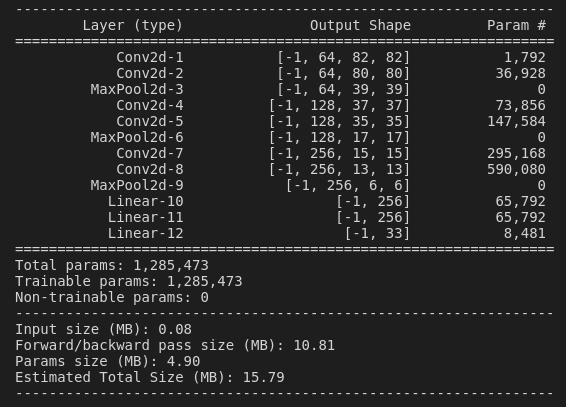
\includegraphics[width=0.7\linewidth]{best_model.png}
    \caption{Best performing model (63 \% test accuracy}
    \label{fig:best_model}
\end{figure}

\begin{itemize}

    \item Weight decay of: \textbf{1e-1}
    \begin{figure}[H]
    \centering
    \begin{minipage}{.5\linewidth}
        \centering
        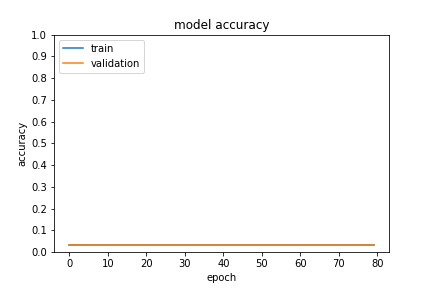
\includegraphics[width=0.9\linewidth]{train_metrics/train_acc_0.png}
        \vspace{-1.0em}
        \caption{Accuracy curves}

    \end{minipage}%
    \begin{minipage}{.5\textwidth}
      \centering
      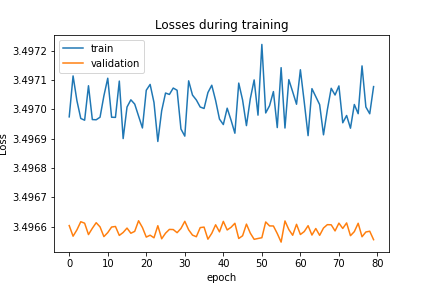
\includegraphics[width=.9\linewidth]{train_metrics/train_loss_0.png}
      \vspace{-1.0em}
      \caption{Loss curves}

    \end{minipage}
    \end{figure}
    
    \item Weight decay of: \textbf{5e-2}
    \begin{figure}[H]
    \centering
    \begin{minipage}{.5\linewidth}
        \centering
        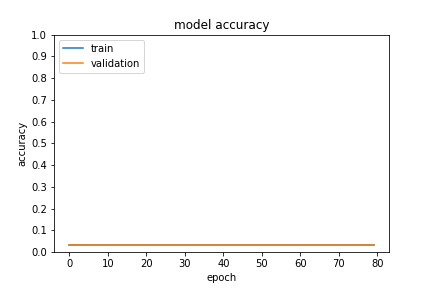
\includegraphics[width=0.9\linewidth]{train_metrics/train_acc_2.png}
        \vspace{-1.0em}
        \caption{Accuracy curves}

    \end{minipage}%
    \begin{minipage}{.5\textwidth}
      \centering
      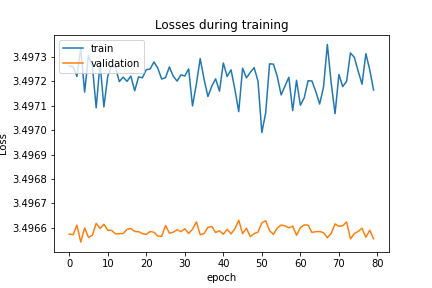
\includegraphics[width=.9\linewidth]{train_metrics/train_loss_2.png}
      \vspace{-1.0em}
      \caption{Loss curves}

    \end{minipage}
    \end{figure}
    
    \item Weight decay of: \textbf{1e-2}
    \begin{figure}[H]
    \centering
    \begin{minipage}{.5\linewidth}
        \centering
        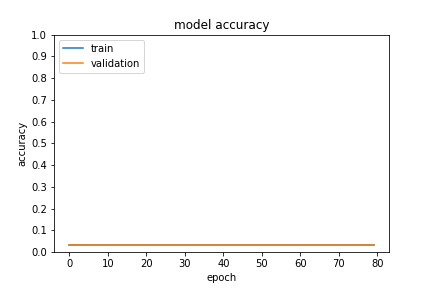
\includegraphics[width=0.9\linewidth]{train_metrics/train_acc_1.png}
        \vspace{-1.0em}
        \caption{Accuracy curves}

    \end{minipage}%
    \begin{minipage}{.5\textwidth}
      \centering
      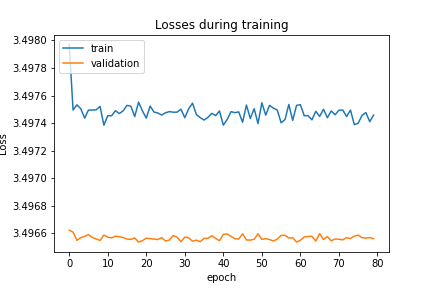
\includegraphics[width=.9\linewidth]{train_metrics/train_loss_1.png}
      \vspace{-1.0em}
      \caption{Loss curves}

    \end{minipage}
    \end{figure}
    
    \newpage
    \item Weight decay of: \textbf{5e-3}
    \begin{figure}[H]
    \centering
    \begin{minipage}{.5\linewidth}
        \centering
        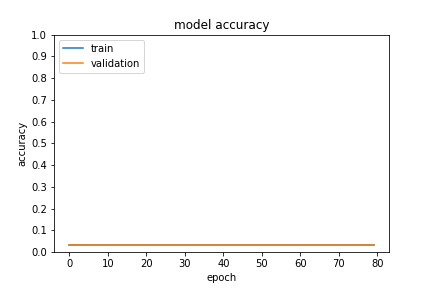
\includegraphics[width=0.9\linewidth]{train_metrics/train_acc_4.png}
        \vspace{-1.0em}
        \caption{Accuracy curves}

    \end{minipage}%
    \begin{minipage}{.5\textwidth}
      \centering
      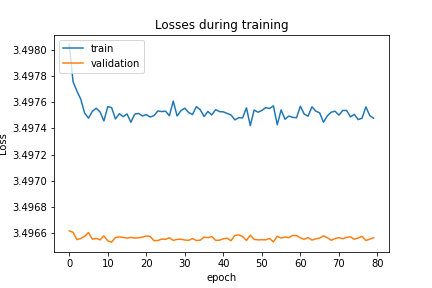
\includegraphics[width=.9\linewidth]{train_metrics/train_loss_4.png}
      \vspace{-1.0em}
      \caption{Loss curves}

    \end{minipage}
    \end{figure}
    
    \item Weight decay of: \textbf{1e-3}
    \begin{figure}[H]
    \centering
    \begin{minipage}{.5\linewidth}
        \centering
        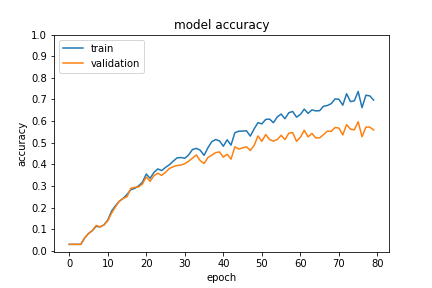
\includegraphics[width=0.9\linewidth]{train_metrics/train_acc_3.png}
        \vspace{-1.0em}
        \caption{Accuracy curves}

    \end{minipage}%
    \begin{minipage}{.5\textwidth}
      \centering
      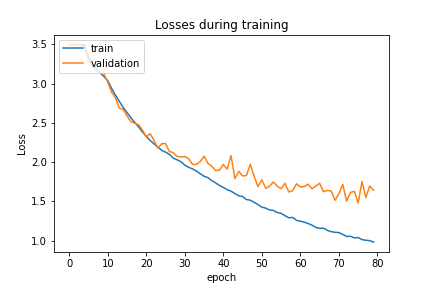
\includegraphics[width=.9\linewidth]{train_metrics/train_loss_3.png}
      \vspace{-1.0em}
      \caption{Loss curves}

    \end{minipage}
    \end{figure}
    
    \item Weight decay of: \textbf{5e-4}
    \begin{figure}[H]
    \centering
    \begin{minipage}{.5\linewidth}
        \centering
        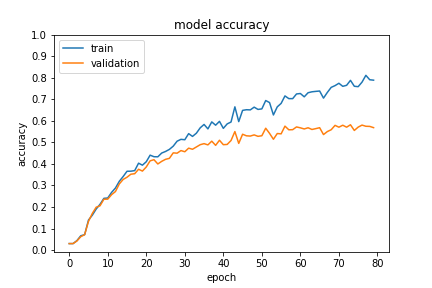
\includegraphics[width=0.9\linewidth]{train_metrics/train_acc_6.png}
        \vspace{-1.0em}
        \caption{Accuracy curves}

    \end{minipage}%
    \begin{minipage}{.5\textwidth}
      \centering
      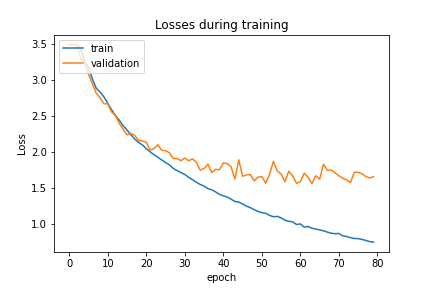
\includegraphics[width=.9\linewidth]{train_metrics/train_loss_6.png}
      \vspace{-1.0em}
      \caption{Loss curves}

    \end{minipage}
    \end{figure}
    
    \newpage    
    \item Weight decay of: \textbf{1e-4}
    \begin{figure}[H]
    \centering
    \begin{minipage}{.5\linewidth}
        \centering
        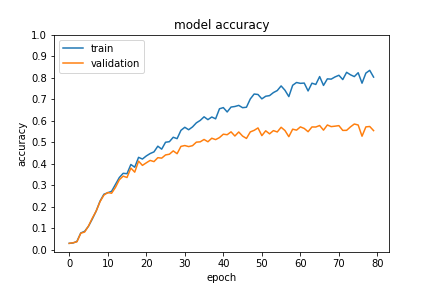
\includegraphics[width=0.9\linewidth]{train_metrics/train_acc_5.png}
        \vspace{-1.0em}
        \caption{Accuracy curves}

    \end{minipage}%
    \begin{minipage}{.5\textwidth}
      \centering
      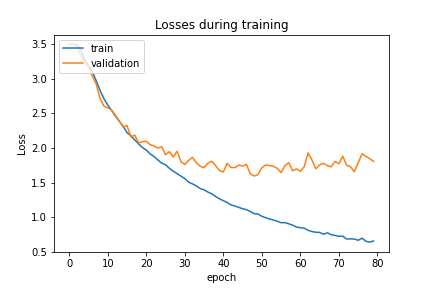
\includegraphics[width=.9\linewidth]{train_metrics/train_loss_5.png}
      \vspace{-1.0em}
      \caption{Loss curves}

    \end{minipage}
    \end{figure}

    \item Weight decay of: \textbf{5e-5}
    \begin{figure}[H]
    \centering
    \begin{minipage}{.5\linewidth}
        \centering
        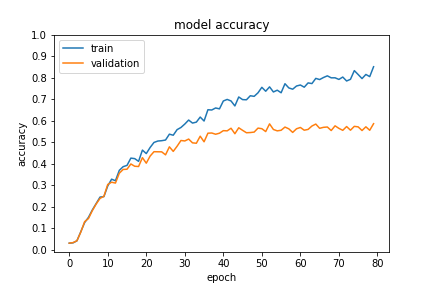
\includegraphics[width=0.9\linewidth]{train_metrics/train_acc_8.png}
        \vspace{-1.0em}
        \caption{Accuracy curves}

    \end{minipage}%
    \begin{minipage}{.5\textwidth}
      \centering
      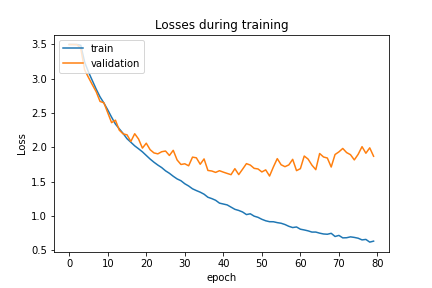
\includegraphics[width=.9\linewidth]{train_metrics/train_loss_8.png}
      \vspace{-1.0em}
      \caption{Loss curves}

    \end{minipage}
    \end{figure}
    
    \item Weight decay of: \textbf{1e-5}
    \begin{figure}[H]
    \centering
    \begin{minipage}{.5\linewidth}
        \centering
        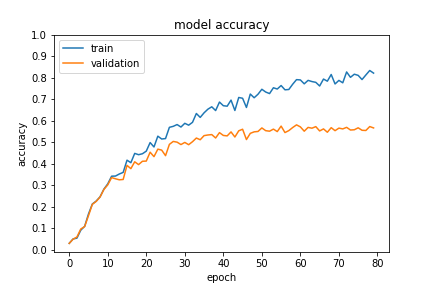
\includegraphics[width=0.9\linewidth]{train_metrics/train_acc_7.png}
        \vspace{-1.0em}
        \caption{Accuracy curves}

    \end{minipage}%
    \begin{minipage}{.5\textwidth}
      \centering
      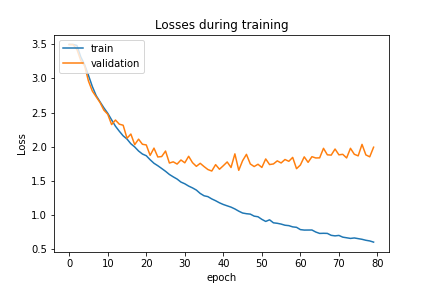
\includegraphics[width=.9\linewidth]{train_metrics/train_loss_7.png}
      \vspace{-1.0em}
      \caption{Loss curves}

    \end{minipage}
    \end{figure}
    
    \newpage
    \item Weight decay of: \textbf{5e-6}
    \begin{figure}[H]
    \centering
    \begin{minipage}{.5\linewidth}
        \centering
        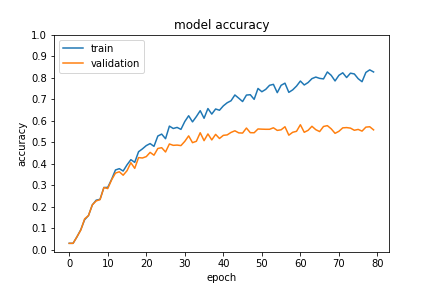
\includegraphics[width=0.9\linewidth]{train_metrics/train_acc_10.png}
        \vspace{-1.0em}
        \caption{Accuracy curves}

    \end{minipage}%
    \begin{minipage}{.5\textwidth}
      \centering
      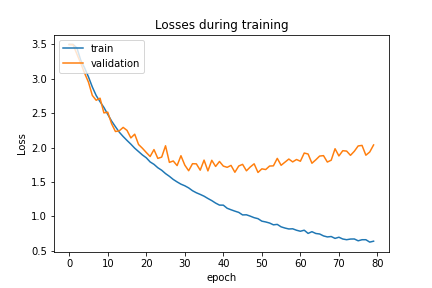
\includegraphics[width=.9\linewidth]{train_metrics/train_loss_10.png}
      \vspace{-1.0em}
      \caption{Loss curves}

    \end{minipage}
    \end{figure}
    
    \item Weight decay of: \textbf{1e-6}
    \begin{figure}[H]
    \centering
    \begin{minipage}{.5\linewidth}
        \centering
        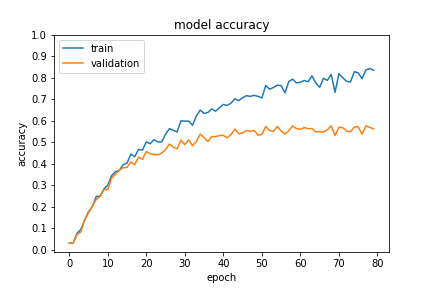
\includegraphics[width=0.9\linewidth]{train_metrics/train_acc_9.png}
        \vspace{-1.0em}
        \caption{Accuracy curves}

    \end{minipage}%
    \begin{minipage}{.5\textwidth}
      \centering
      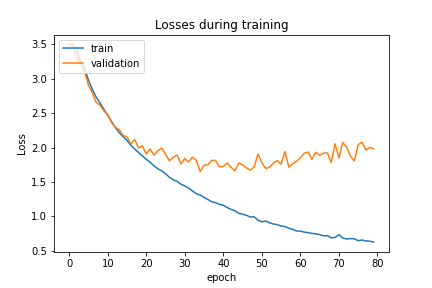
\includegraphics[width=.9\linewidth]{train_metrics/train_loss_9.png}
      \vspace{-1.0em}
      \caption{Loss curves}

    \end{minipage}
    \end{figure}
    
\end{itemize}

\begin{table}[h!]
\begin{center}
\begin{tabular}{ |c|c|c|} 
 \hline
 weight decay & \% Training Accuracy & \% Test accuracy\\ 
 \hline
 1e-1 & 3.03 & 3.03  \\ 
 \hline
 5e-2 & 3.03  & 3.03  \\ 
\hline
 1e-2 & 3.03  & 3.03  \\ 
\hline
 5e-3 & 3.03  & 3.03  \\
\hline
 1e-3 & 73.7 & 59.7 \\
\hline
 5e-4 & 81.08 & 58.15\\
\hline
 1e-4 & 83.39 & \textbf{58.45} \\
\hline
 5e-5 & 85.05 & \textbf{58.58}\\
\hline
 1e-5 & 83.31 & 58.06 \\
\hline
 5e-6 & 83.61  & 58.12 \\
\hline
 1e-6 & 84.26  & 57.61  \\
\hline
\end{tabular}
\caption{Final results by varying weight decay }
\end{center}
\end{table}

\newpage
% Summary and Conclusions
\subsubsection{Summary and Conclusions}

One way for Regularization, which is a way to penalize complexity is to add all our parameters (weights) to our loss function. It usually doesn't quite work well because some parameters are positive and some are negative and even if we add the squares of all the parameters to our loss function, the loss would get so huge for large models that the best model would be to set all the parameters to 0.\\

\noindent
To prevent this from happening, we multiply the sum of squares with another smaller number. This number is called the weight decay or $wd$.
Our loss function for our network looks as follows:
\begin{equation}
 Loss = CrossEntropyLoss(y_{pred}, y) + wd * sum(w^2)
\end{equation}
We can understand for the results above that if we have too much weight decay, then no matter how much you train, the model will never quite fit well and converge whereas if we have too little weight decay, then we can still train well, we just need to monitor when the model starts over-fitting (ref Table 1).\\

\noindent
This can especially be seen for the high weight decay values 1e-1, 5e-2, 1e-2, 5e-2 where the model is not training at all and the model is stuck, since the modal is being very heavily penalized and the model parameters just tend to zero. As the weight decay parameter decrease, we see its positive effects. However as it goes less than 1e-5, we see that the model tends to take more time to converge, hence some value around the range of (1e-4,5e-5) looks ideal.

\section{Part-B}

Since this part is a written assignment, the solutions were scanned and have been attached in Q2 folder.

\end{document}
